% HMC Math dept HW template example
% v0.04 by Eric J. Malm, 10 Mar 2005
\documentclass[12pt,letterpaper,boxed,cm]{hmcpset}

% set 1-inch margins in the document
\usepackage[margin=1in]{geometry}
\usepackage{mathtools}
\usepackage{mathrsfs}
% include this if you want to import graphics files with /includegraphics
\usepackage{graphicx}
\usepackage{cases}
\usepackage{hyperref}
\usepackage{siunitx}
\usepackage{tikz}
\usepackage{cases}
\usetikzlibrary{arrows}

% info for header block in upper right hand corner
\name{Name: ~~~~~~~~~~~~~~~~~~~~~~~}
\class{Physics 51}
\assignment{Homework \#9}
\duedate{October 3, 2016}

\newcommand{\ev}[2]{\Big|_{#1}^{#2}}
\newcommand{\evv}[2]{\Big|_{#1}^{#2}}
\newcommand{\set}[1]{\left\{#1\right\}}
\newcommand{\s}[1]{\sqrt{#1}}
\newcommand{\f}[2]{\frac{#1}{#2}}
\newcommand{\p}[2]{\frac{\partial #1}{\partial #2}}
\providecommand{\t}[1]{\text{#1}}
\providecommand{\span}[1]{\text{span}\left(#1\right)}
\providecommand{\set}[1]{\left\{#1\right\}}
\providecommand{\l}[0]{\left}
\providecommand{\r}[0]{\right}
\newcommand{\m}[1]{\begin{matrix}#1\end{matrix}}
\newcommand{\bm}[1]{\begin{bmatrix}#1\end{bmatrix}}
\renewcommand{\bf}[1]{\mathbf{#1}}
\newcommand{\pn}[1]{\left( #1 \right)}
\newcommand{\abs}[1]{\left| #1 \right|}
\newcommand{\bk}[1]{\left[ #1 \right]}
\newcommand{\cis}[1]{\pn{\cos\pn{#1} + i\sin\pn{#1}}}
\newcommand{\cisi}[1]{\pn{\cos\pn{#1} - i\sin\pn{#1}}}
\renewcommand{\Im}[1]{\text{Im}\pn{#1}}
\renewcommand{\Re}[1]{\text{Re}\pn{#1}}
\renewcommand{\k}[0]{\f{1}{4\pi\epsilon_0}}
\renewcommand{\part}[1]{\vspace{1em}\noindent(#1)}

\makeatletter
\renewcommand*\env@matrix[1][*\c@MaxMatrixCols c]{%
  \hskip -\arraycolsep
  \let\@ifnextchar\new@ifnextchar
  \array{#1}}
\makeatother
\begin{document}
\problemlist{32-P4, 32-P18, 32-E1*, 33-E24}

\begin{problem}[32-P4]
	A beam of electrons whose kinetic energy is $K$ emerges from a thin-foil "window" at the end of an accelerator tube. There is a metal plate a distance $d$ from this window and at right angles to the direction of the emerging beam (see Fig. 32-38). 
	\begin{enumerate}
		\item[(a)] Show that we can prevent the beam from hitting the plate if we apply a magnetic field $B$ such that 
		\[
			B \ge \sqrt{\f{2mK}{e^2d^2}},
		\]
		in which $m$ and $e$ are the electron mass and charge.
		\item[(b)] How should $B$ be oriented?
	\end{enumerate}
	\begin{center}
		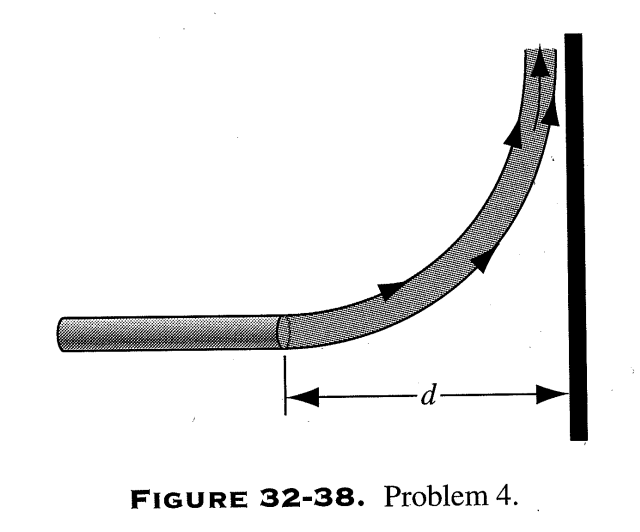
\includegraphics[scale=0.7]{01.png}	
	\end{center}
\end{problem}
\begin{solution}
\end{solution}
\newpage

\begin{problem}[32-P18]
	Figure 32-44 shows a wire ring of radius $a$ at right angles to the general direction of a radially symmetric diverging magnetic field. The magnetic field at the ring is everywhere of the same magnitude $B$, and its direction  at the ring is everywhere at an angle $\theta$ with a normal to the plane of the ring. The twisted lead wires have no effect on the problem. Find the magnitude and direction of the force the field exerts on the ring if the ring carries a current $i$ as shown in the figure.
	\begin{center}
		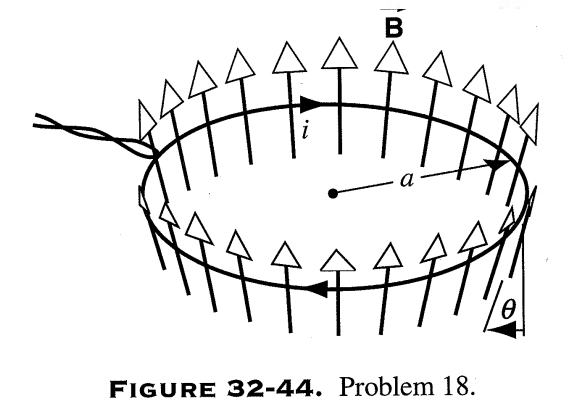
\includegraphics[scale=0.7]{02.png}	
	\end{center}
\end{problem}
\begin{solution}
\end{solution}
\newpage

\begin{problem}[32-E1*]
	Four particles follow the paths shown in Fig 32-33 as they pass through the magnetic field there. What can one conclude about the charge of each particle.
	\begin{center}
		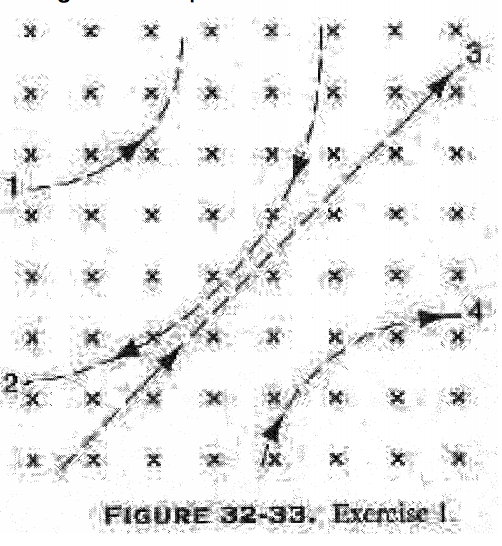
\includegraphics[scale=0.7]{03.png}	
	\end{center}
\end{problem}
\begin{solution}
\end{solution}


\newpage
\begin{problem}[33-E24]
	Figure 46 shows a long wire carrying a current $i$. The rectangular loop carries a current $i_2$. Calculate the resultant force acting on the loop. Assume that $a = \SI{1.10}{cm}$, $b = \SI{9.20}{cm}$, $L = \SI{32.3}{cm}$, $i_1 = \SI{28.6}{A}$, and $i_2 = \SI{21.8}{A}$.	
	\begin{center}
		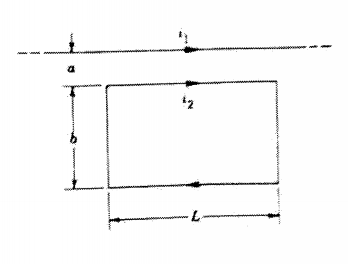
\includegraphics[scale=1.4]{04.png}	
	\end{center}
\end{problem}
\begin{solution}
\end{solution}

\end{document}